\section{Inspiracja}
W 2003 roku niejaki Barrett Lyon, informatyk oraz artysta, postawił sobie za cel stworzenie wiernego odwzorowania połączeń między komputerami w sieci Internet. Wizualizacja grafu miała być zrealizowana za pomocą kolorowych linii oraz punktów. W ten sposób, w październiku 2003 roku powstał open source-owy Projekt Opte. Głównym celem tego projektu było zilustrowanie wciąż szybko rozwijającego się Internetu oraz wyróżnienie regionów, które w tamtych czasach doświadczały gwałtowny wzrost łączności z Internetem.

Projekt szybko zyskał dużą popularność, a jeden z efektów końcowych można było zobaczyć na żywo w Muzeum Sztuki Nowoczesnej w Nowym Jorku. Przykładową wizualizację zaprezentowano na \ref{opte-project}.

Twórca Opte Project w artykule dla Time \cite{OpteProject:Time} krótko podsumował swoją motywację:

\begin{center}

\hyphenblockcquote{USenglish}{OpteProject:Time}{
	The Internet is really big, very connected and extremely complex. \linebreak
	It’s this whole world you can’t see. That’s the fun part of visualizing it.
}
\end{center}


\begin{figure*}[!h]
	\begin{center}
		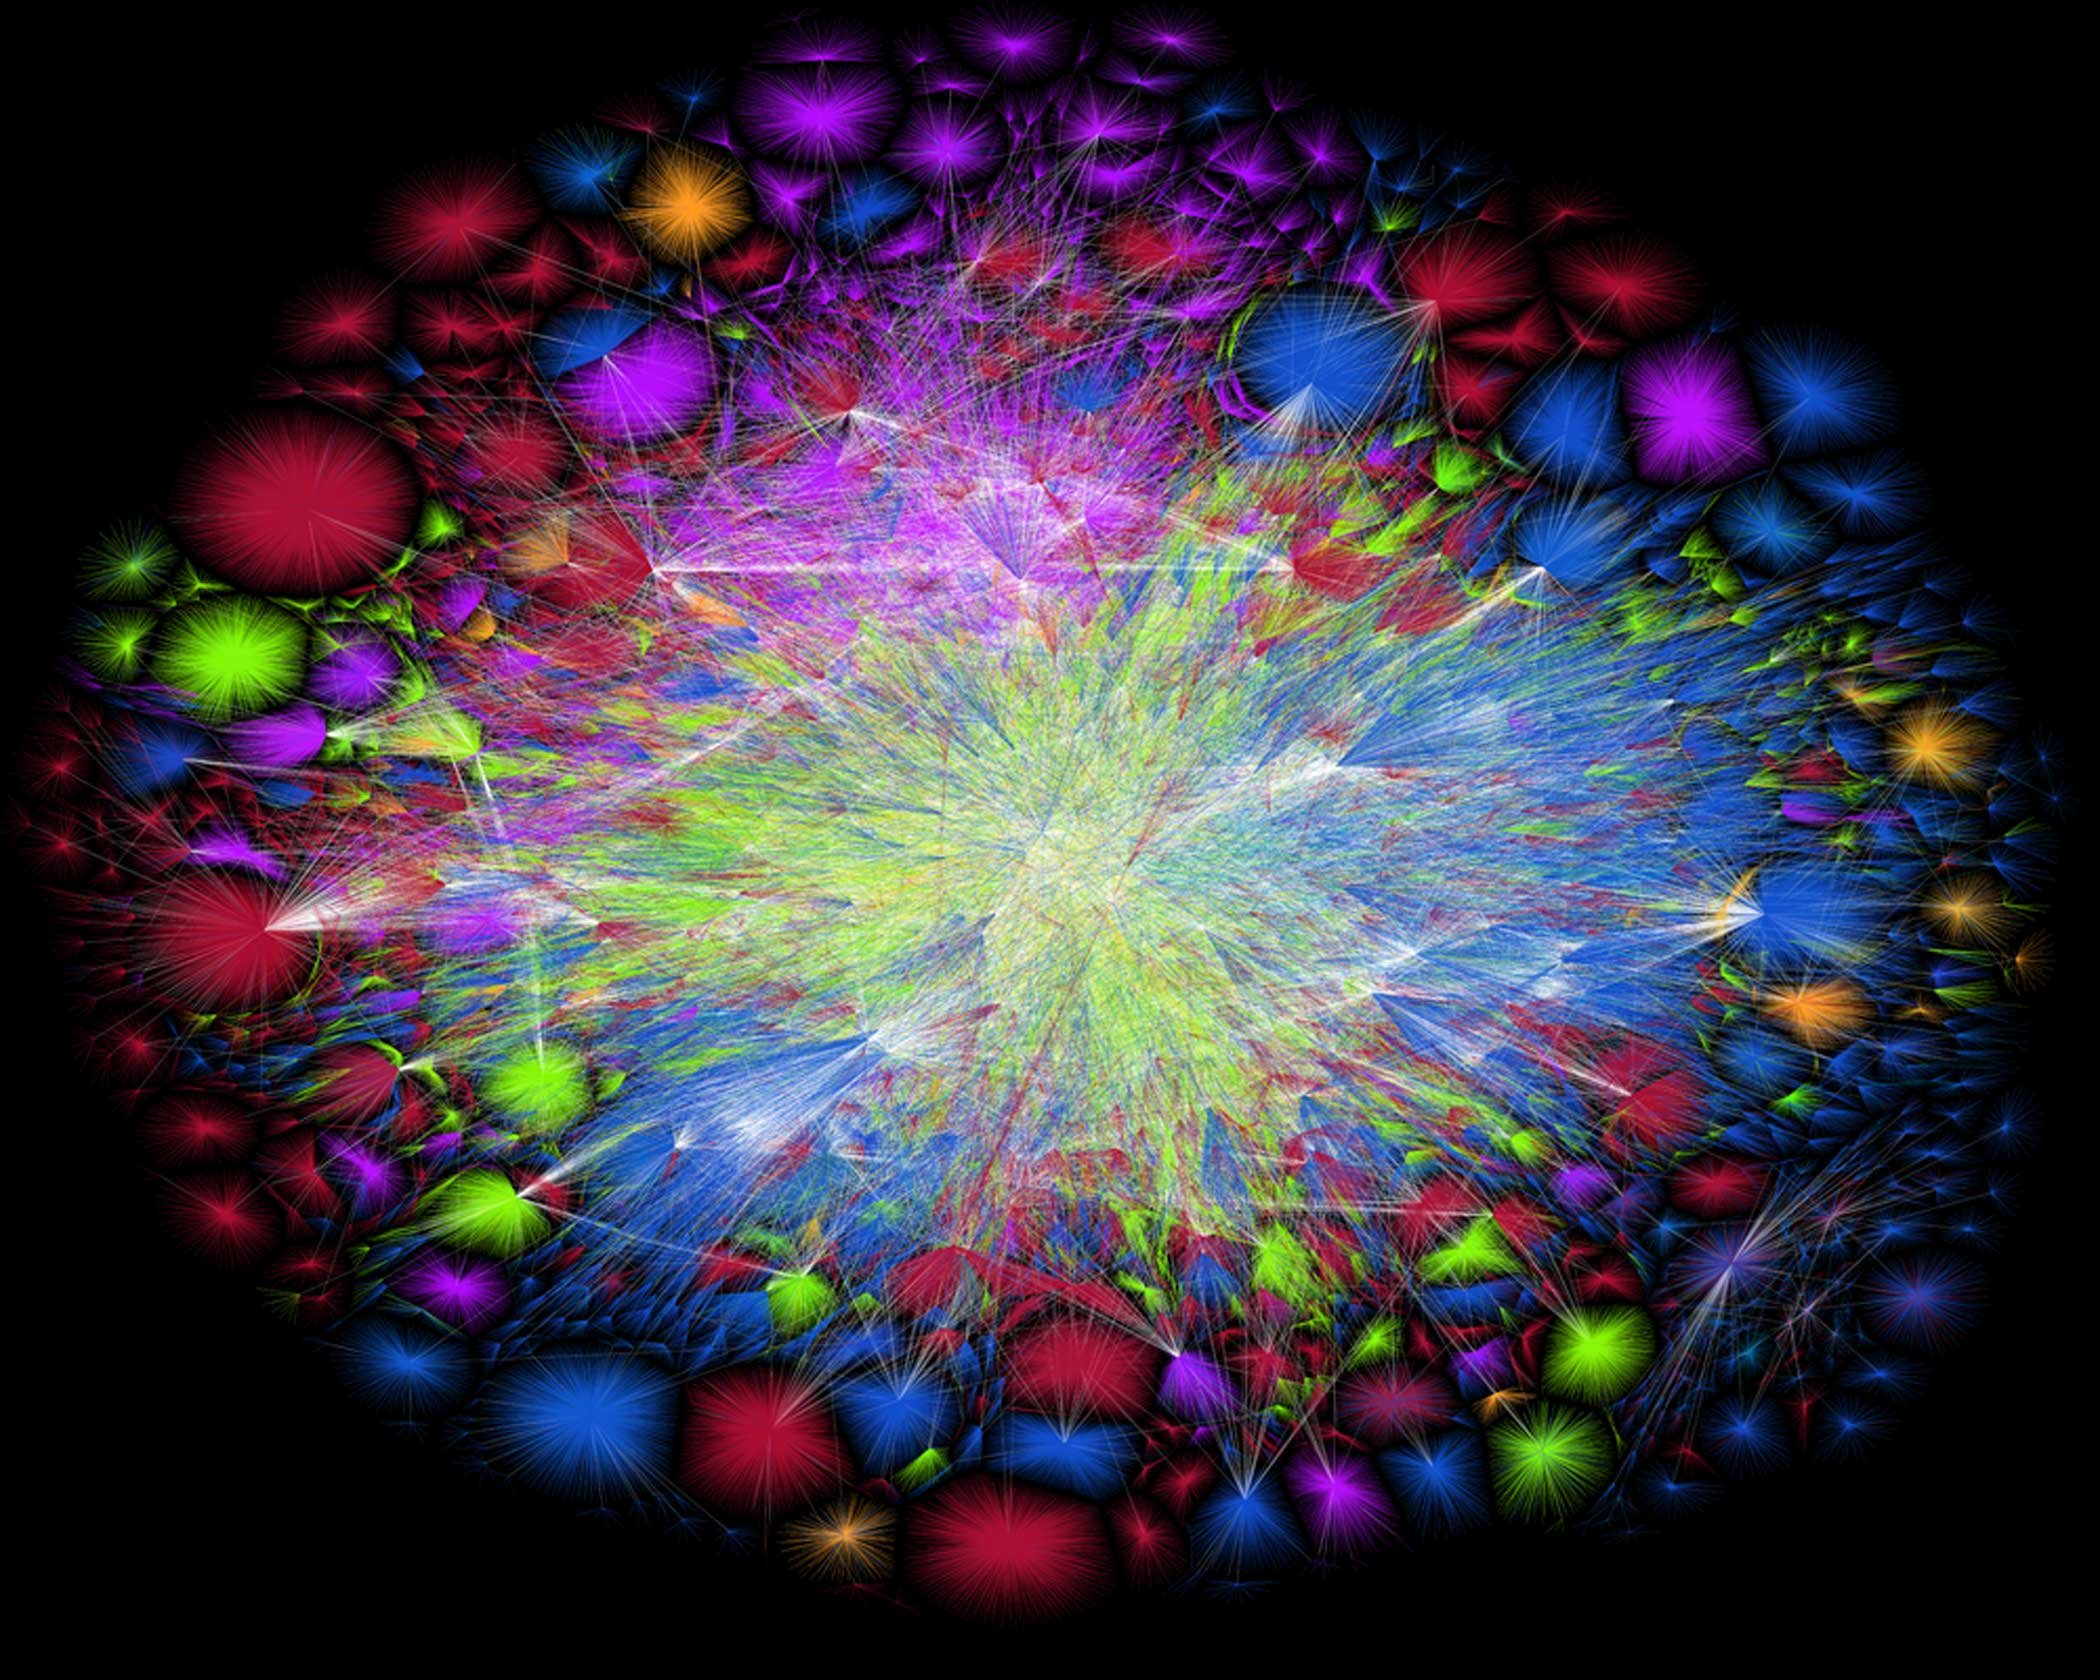
\includegraphics[width=0.6\textwidth]{\chapterPath/img/opte-project.jpg}
		\caption{Jedna z wizualizacji stworzona przez Opte Project}
		\label{opte-project}
	\end{center}
\end{figure*}
